\begin{itemize}
	\subsubsection{Overview of mini-batch gradient descent}
	\subsubsection{Reminder: The error surface for a linear neuron}
	\item The error surface lies in a space with a horizontal axis for each weight and one vertical axis for the error
	\begin{itemize}
		\item For a linear neuron with a squared error, it is a quadratic bowl
	\end{itemize}

	\item For multi-layer, non-linear nets the error surface is much more complicated
	\begin{itemize}
		\item But locally, a piece of a quadratic bowl is an approximation
	\end{itemize}

	\subsubsection{Convergence speed of full batch learning when the error surface is a quadratic bowl}
	\item Going downhill reduces the error, but the direction of steepest descent does not point at the minimum unless the ellipse is a circle
	\item The gradient is big in the direction in which we only want to travel a small distance (larger axis of ellipse, where we only want to travel a small distance)
	\item The gradient is small in the direction in which we want to travel a large distance (towards the center on the smaller axis).
	\item Even for non-linear multi-layer nets, the error surface is locally quadratic, so the same speed issues apply
	\begin{center}
		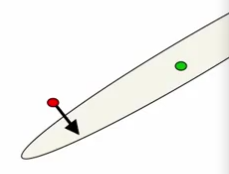
\includegraphics[scale=0.9]{sections/6/ellipse.png}
	\end{center}

	\subsubsection{How the learning goes wrong}
	\item If the learning rate is big, the weights slosh to and fro acoss the ravine (this can diverge)
	\begin{center}
		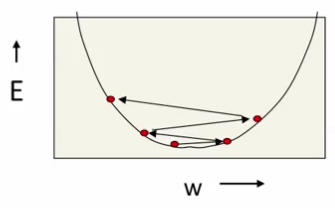
\includegraphics[scale=0.9]{sections/6/div.png}
	\end{center}

	\item What we want:
	\begin{itemize}
		\item Move quickly in directions with small but consistent gradients
		\item Move slowly in directions with big but inconsistent gradients
	\end{itemize}
	
	\subsubsection{Stochastic gradient descent}
	\item If the dataset is highly redundant, the gradient on the first half is almost identical to the gradient on the second half
	\item So instead of computing the full gradient, update the weights using the gradient on the first half and then get a gradient for the new weights on the second half
	\item An extreme version of this approach updates weights after each case. It's called ``online.''
	\item Mini-batches are usually better than online (10, 100, 1000)
	\begin{itemize}
		\item Less computation is used updating the weights
		\item Computing the gradient for many cases simultaneously uses matrix-matrix multiplies which are very efficient, especially on GPUs
	\end{itemize}

	\item Mini-batches need to be balanced for classes
	\item Ideal would be exactly same number of each class type in each mini-batch
	\item Avoid mini-batches that are very uncharacterstic of the data (e.g., all the same class)

	\subsubsection{Two types of learning algorith}
	\item If we use the full gradient computed from all the training cases, there are many clever ways to speed up learning (e.g., non-linear conjugate gradient)
	\item The optimization community has studied the general problem of optimizing smooth non-linear functions for many years
	\item Multilayer neural nets are not typical of the problems they study so their methods may need a lot of adaptation.
	\item For large neural networks with very large and highly redundant training sets, it is nearly always best to use mini-batch learning

	\subsubsection{A basic mini-batch gradient descent algorithm}
	\item Guess an initial learning rate
	\begin{itemize}
		\item If the error keeps getting worse or oscillates wildly, reduce the learning rate
		\item If the error is falling fairly consistently but slowly, increase the learning rate
	\end{itemize}
	\item Write a simple program to autmate this way of adjusting the learning rate
	\item Towards the end of mini-batch learning it always nearly helps to turn down the learning rate
	\begin{itemize}
		\item This removes fluctuations in the final weights caused by the variations between mini-batches
	\end{itemize}
	\item Turn down the learning rate when the error stops decreasing
	\item Use the error on a separate validation set
\end{itemize}